\documentclass[10pt,a4paper,twocolumn]{article}
\usepackage[T1]{fontenc}
\usepackage[utf8]{inputenc}
\usepackage{mathptmx}
\usepackage[a4paper,top=2.2cm,bottom=2.5cm,left=1.8cm,right=1.8cm,columnsep=0.65cm]{geometry}
\usepackage{amsmath}
\usepackage{graphicx}
\usepackage{booktabs}
\usepackage[font=small,labelsep=colon,skip=4pt]{caption}
\usepackage{titlesec}
\usepackage{microtype}
\usepackage{cite}
\usepackage{url}
\usepackage[hidelinks]{hyperref}

\titleformat{\section}{\normalfont\bfseries\centering}{\thesection.}{0.5em}{\MakeUppercase}
\titlespacing*{\section}{0pt}{10pt plus 2pt}{5pt}
\titleformat{\subsection}{\normalfont\bfseries}{\thesubsection.}{0.5em}{}
\titlespacing*{\subsection}{0pt}{7pt plus 2pt}{3pt}
\setlength{\abovedisplayskip}{5pt plus 2pt}
\setlength{\belowdisplayskip}{5pt plus 2pt}
\setlength{\textfloatsep}{10pt plus 2pt}

\newcommand{\Hz}{\,\mathrm{Hz}}
\newcommand{\dB}{\,\mathrm{dB}}
\newcommand{\s}{\,\mathrm{s}}
\newcommand{\ms}{\,\mathrm{ms}}
\newcommand{\ct}{\,\mathrm{cents}}
\renewcommand{\Im}{\operatorname{Im}}
\newcommand{\sst}{\operatorname{s}}

\hypersetup{pdftitle={Overtone Spiral: measuring the sustained partials of struck singing bowls},
            pdfauthor={Claude (Anthropic) and Michael Kopp}}

\begin{document}

\twocolumn[{%
\begin{center}
{\Large\bfseries OVERTONE SPIRAL: MEASURING THE SUSTAINED PARTIALS\\[2pt] OF STRUCK SINGING BOWLS\par}
\vspace{12pt}
{\large Claude (Anthropic)\textsuperscript{$*$}\qquad Michael Kopp\textsuperscript{$\dagger$}\par}
\vspace{6pt}
October 2, 2026
\end{center}
\vspace{10pt}
}]

\begingroup
\renewcommand{\thefootnote}{\fnsymbol{footnote}}
\footnotetext[1]{Claude Opus 5.5, model string \texttt{claude-opus-5-5}, run as an agent with file, shell and browser access at extra reasoning effort. Work carried out in October 2026.}
\footnotetext[2]{Corresponding author: \texttt{mkopp911@gmail.com}}
\endgroup

\begin{center}\bfseries ABSTRACT\end{center}
\vspace{-4pt}
\noindent
We describe a method, and its implementation as a single web page, for measuring the fundamental and the dominant sustained partials of a struck idiophone, the crystal singing bowl in particular, from a recording or from a microphone, and for displaying them on a spiral with one turn per octave. The method chooses its own analysis window: attacks are detected in two high-passed bands, the ring-out after each attack is analysed as a candidate, and the candidate whose confident partials have the highest signal-to-noise ratios is retained. Within the window every frame is analysed on its own: the frequency of each bin is obtained by time-frequency reassignment with the derivative of the Blackman--Harris window, peaks are validated by the agreement of the reassigned frequencies across the main lobe, and peaks are linked into partials. Each partial receives a confidence, combining signal-to-noise ratio, duration, continuity and frequency stability, and a standard uncertainty. Split modes, which make the partials of a bowl beat, are resolved on a zoom spectrum of the ring-out; when they decay too fast for that, their beat is measured from the periodicity of the amplitude envelope and the uncertainty is widened accordingly. No phase information is carried from one frame to the next. On a synthetic ring-out with widely split modes, five partials and both modes of each pair are recovered to $10^{-5}\Hz$; with splits, decay rates and noise close to those of a recorded bowl, the main modes of the three resolved pairs are recovered to $0.03$~cents. On the recorded bowl, three partials are resolved as split pairs, with standard uncertainties of $0.06$ to $0.14$~cents, and a fourth, which beats at $3\Hz$ but decays too fast to be resolved, is listed with an uncertainty of $1.5$~cents.

\section{Introduction}

A struck singing bowl sounds a small number of strong, slowly decaying, inharmonic partials. The lowest is usually taken as the note of the bowl, but the upper partials distinguish one bowl from another and decide how bowls sound together. Describing a bowl therefore means measuring a handful of partials to a fraction of a cent, naming them on the tempered scale, and saying which of them are clearly heard. Two properties of the instrument complicate the task: the partials decay, and the degenerate mode pairs of a nearly axisymmetric shell are split by small asymmetries into close pairs that beat~\cite{FletcherRossing,Inacio,Terwagne}.

The Snail~\cite{HelieSnail,HelieTimbre} displays the spectrum on a spiral with one turn per octave, so that the pitch classes lie on radial lines and octaves on the same radius. Its frequency precision comes from the demodulated phase of the short-time Fourier transform (STFT), the phase of each bin less that of a reference oscillation at the bin frequency: a low-pass filtered indicator of the constancy of this phase across frames sharpens the representation, and its change over one hop gives a frequency deviation~\cite{HelieTimbre,HeliePatent}. The Snail is a real-time display for performers. Sinusoidal modelling~\cite{McAulay,PARSHL,SMS} tracks partials through successive spectra, and the reassignment method~\cite{Kodera76,Kodera78,AugerFlandrin} concentrates a time-frequency representation on the instantaneous frequencies of its components.

This paper describes a method that produces a list of measured partials with a statement of how far each can be trusted, together with a spiral display of the spectrum from which they were measured. Its elements are:
(i)~an automatic choice of the analysis window, the free ring-out after a strike (Section~\ref{sec:window});
(ii)~a frequency for every bin of every frame by reassignment computed within that frame (Section~\ref{sec:frame});
(iii)~partials with a confidence and an uncertainty, and the rejection of background tones (Section~\ref{sec:partials});
(iv)~the resolution of split modes and the measurement of their beat rate (Section~\ref{sec:split});
(v)~a spiral display of the reassigned spectrum (Fig.~\ref{fig:spiral}), and an audibility class for each partial (Section~\ref{sec:display}).
No frequency estimate in Sections~\ref{sec:frame}--\ref{sec:partials} uses phase information from more than one frame, and the zoom spectrum of Section~\ref{sec:split} is the Fourier transform of one segment. Section~\ref{sec:eval} evaluates the method on synthetic signals and on a recorded bowl, and Section~\ref{sec:snail} compares it with the Snail. The implementation is a single HTML file that runs in a web browser.

\begin{figure}[t]
\centering
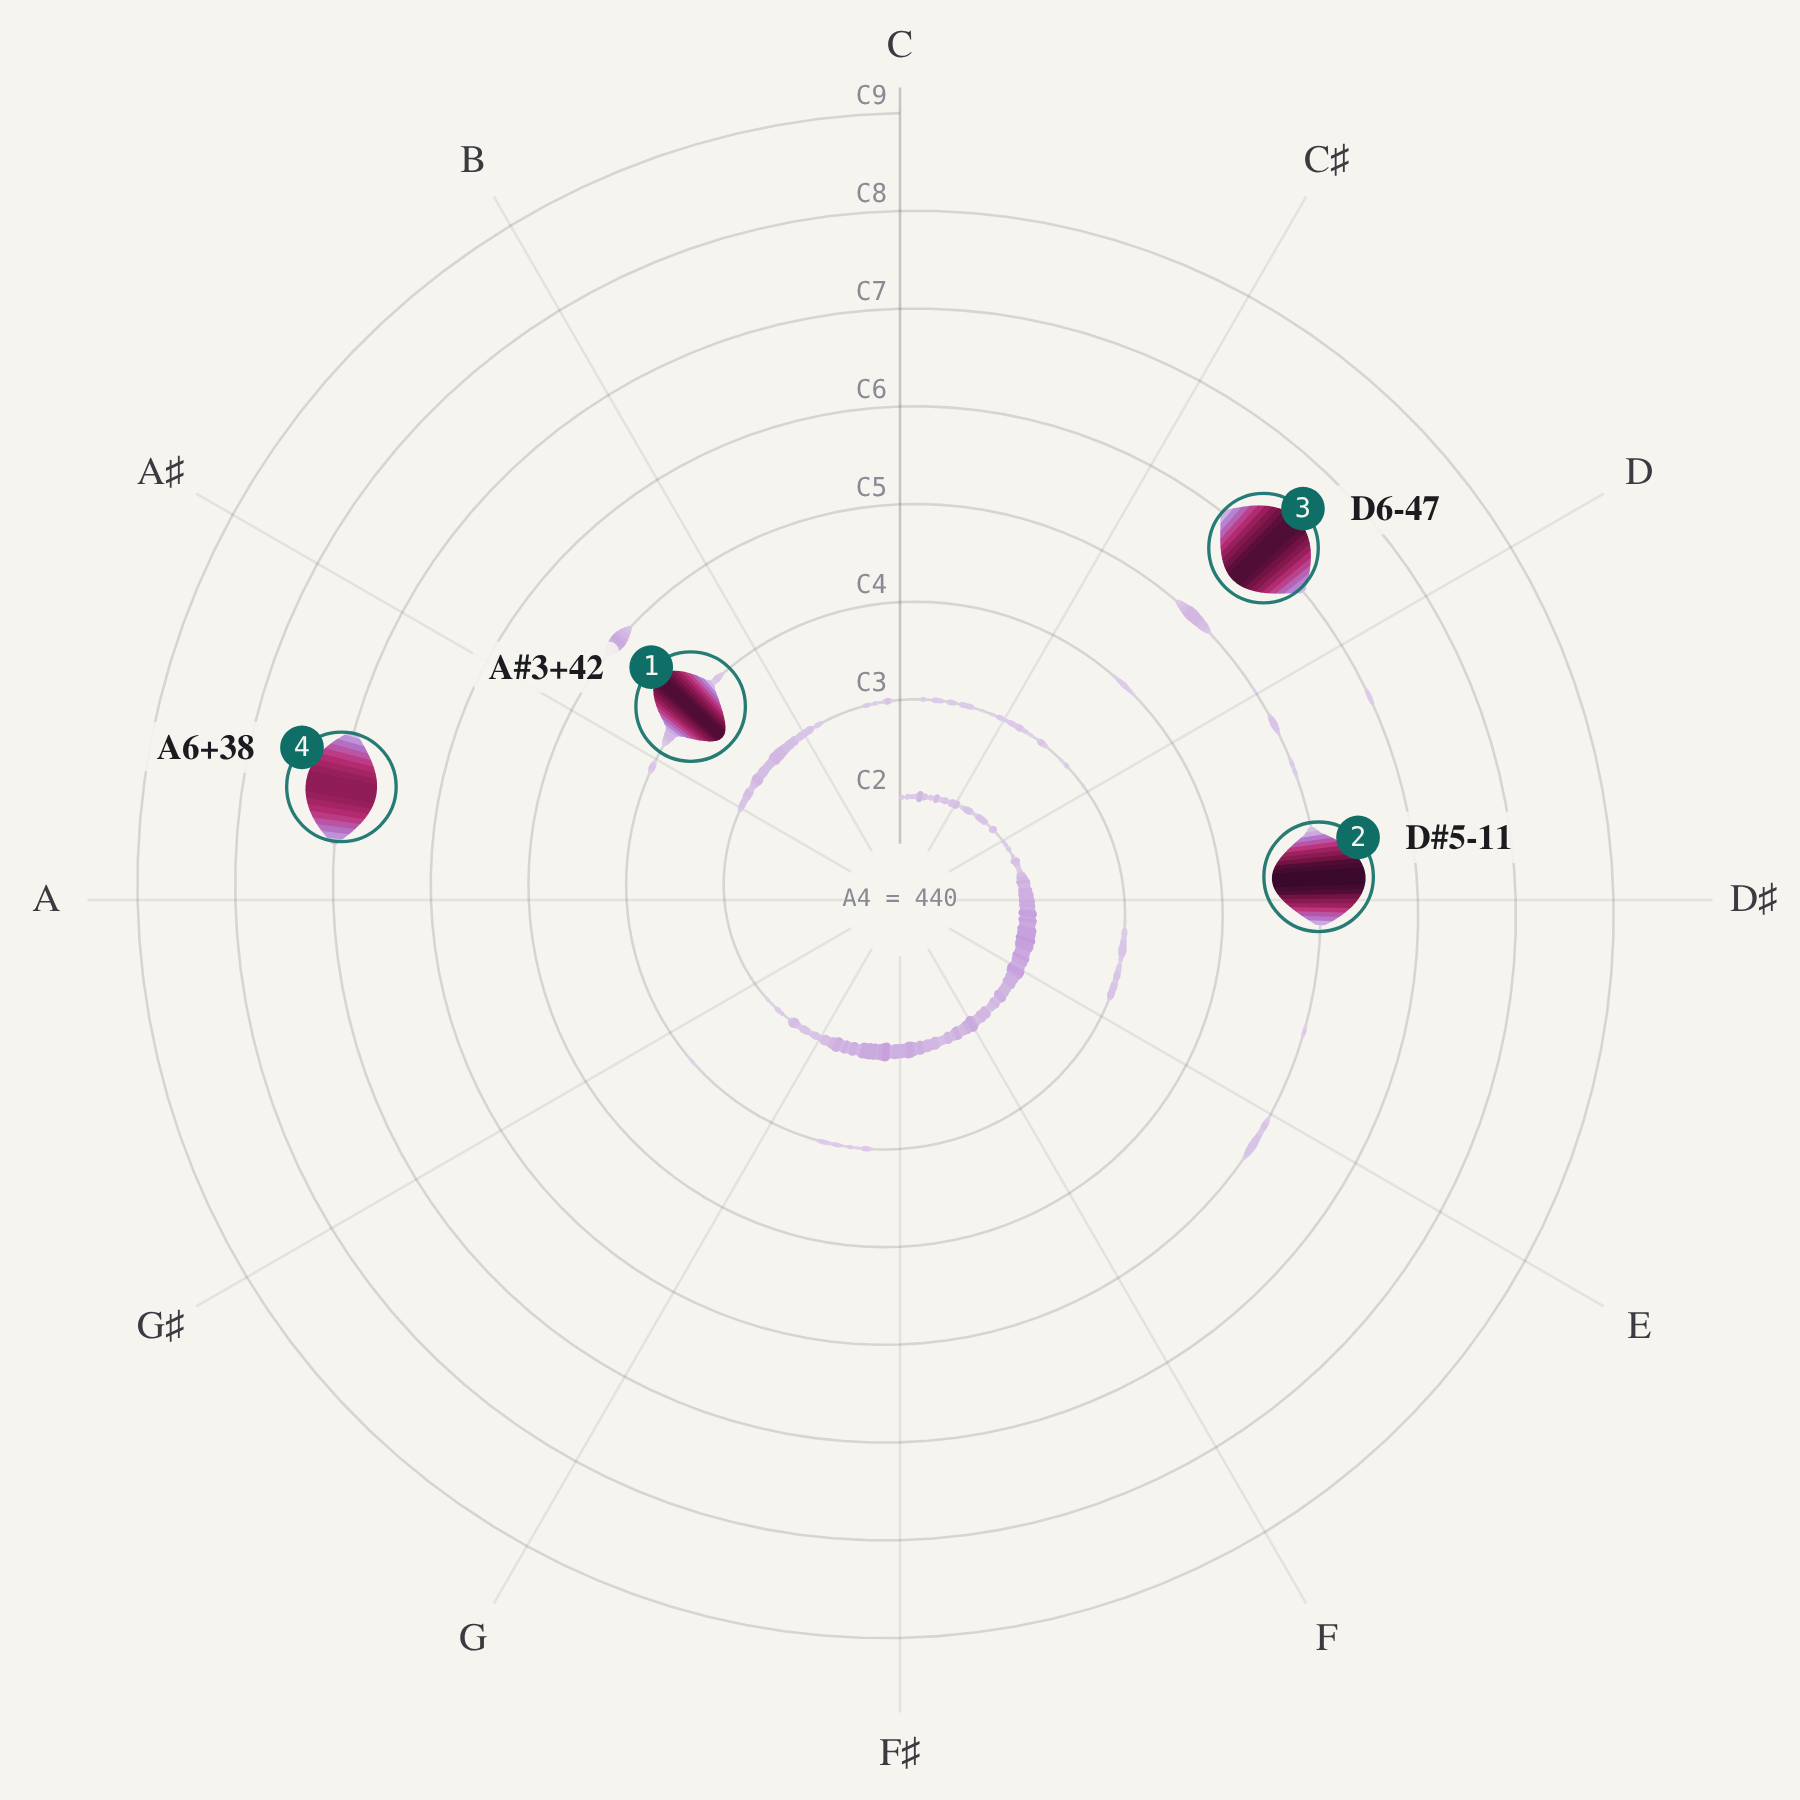
\includegraphics[width=\columnwidth]{fig_spiral.png}
\caption{The spiral display for the recorded bowl of Section~\ref{sec:bowl}: reassigned spectrum of the window $18.62$--$23.80\s$ (display range $60\dB$) and the four listed partials, numbered as in Table~\ref{tab:bowl}. One turn is one octave, from C2 at the centre to C9; equal-tempered pitch classes lie on the radial lines.}
\label{fig:spiral}
\end{figure}

\section{Signal model and notation}
\label{sec:model}

A signal $x[n]$ sampled at $f_s$ is observed. After a strike at $t_0$ it is modelled as
\begin{equation}
x(t) = \sum_p a_p\, e^{-(t-t_0)/\tau_p} \cos\bigl(2\pi f_p (t-t_0) + \varphi_p\bigr) + b(t) + e(t),
\label{eq:model}
\end{equation}
a sum of exponentially decaying partials, a steady background $b$ (mains hum, electronics) and noise $e$. A split mode is a pair $f_p, f_{p'}$ a fraction of a hertz to a few hertz apart, whose sum beats at $|f_p-f_{p'}|$.

A frequency $f$ is named by its MIDI number $m = 69 + 12\log_2(f/f_{\mathrm{A4}})$, with $f_{\mathrm{A4}} = 440\Hz$ by default~\cite{ISO16}: the nearest integer $\bar m$ gives the note name and octave, and $c = 100(m-\bar m)$, rounded, the deviation in cents. A partial at $238.87\Hz$ ($m = 58.42$) is written \texttt{A\#3+42}.

The STFT of frame $\ell$ is
\begin{equation}
X_h[\ell,k] = \sum_{n=0}^{N-1} x[\ell H + n]\, h[n]\, e^{-2\pi i k n/N},
\label{eq:stft}
\end{equation}
with $N = 2^{\lceil \log_2(0.17 f_s)\rceil}$, i.e.\ $N = 8192$ at both $44.1$ and $48\,\mathrm{kHz}$ ($186$ and $171\ms$), hop $H = N/16$, and bin spacing $f_s/N = 5.86\Hz$ at $48\,\mathrm{kHz}$; frames of half and twice this length are available as options. The window is the four-term Blackman--Harris window~\cite{Harris},
\begin{equation}
h[n] = a_0 - a_1 \cos\tfrac{2\pi n}{N} + a_2 \cos\tfrac{4\pi n}{N} - a_3 \cos\tfrac{6\pi n}{N},
\label{eq:bh}
\end{equation}
with $a_0 = 0.35875$, $a_1 = 0.48829$, $a_2 = 0.14128$ and $a_3 = 0.01168$. Its highest side lobe lies $92\dB$ below the main lobe, which extends $\pm 4$ bins.

\section{Frame analysis}
\label{sec:frame}

\subsection{Reassigned frequency}

Kodera, Gendrin and de Villedary~\cite{Kodera76,Kodera78} proposed to move each value of the spectrogram to the centre of gravity of the signal energy around it, and Auger and Flandrin~\cite{AugerFlandrin} showed that the coordinates of that centre of gravity follow from two further STFTs, made with windows derived from $h$. For the frequency coordinate, let $X_h(t,\omega) = \int x(s)\, h(s-t)\, e^{-i\omega s}\, ds$ and let $X_{\mathcal{D}h}$ be the same transform with the window $\mathcal{D}h = dh/dt$. The reassigned frequency is
\begin{equation}
\hat\omega(t,\omega) = \omega - \Im\left\{ \frac{X_{\mathcal{D}h}(t,\omega)}{X_h(t,\omega)} \right\}.
\label{eq:reass}
\end{equation}
(With the window written $h(t-s)$, as in~\cite{AugerFlandrin}, the sign of the correction is reversed.) For a damped complex exponential $x(s) = e^{(-\lambda + i\omega_0)s}$, integration by parts gives $X_{\mathcal{D}h} = (\lambda - i\omega_0 + i\omega)\,X_h$, up to a boundary term that vanishes when $h$ vanishes at both ends; then $\hat\omega = \omega_0$ at every $(t,\omega)$, whatever the damping $\lambda$. The reassigned frequency of a decaying partial is therefore not biased by its decay, which suits the ring-out of a struck bowl. The quantity~\eqref{eq:reass} is the instantaneous frequency of the band-pass signal of the bin~\cite{Kodera78,AugerFlandrin,FulopFitz}. The phase vocoder~\cite{FlanaganGolden} estimates it from the phase difference of successive frames, and the Snail from the demodulated phase~\cite{HelieTimbre}; a related single-frame estimator uses the spectrum of the derivative of the signal~\cite{DesainteCatherine}. Here it is computed within one frame from the derivative of the window.

In discrete form, with the derivative of~\eqref{eq:bh} per sample,
\begin{equation}
\mathcal{D}h[n] = \tfrac{2\pi}{N}\Bigl(a_1 \sin\tfrac{2\pi n}{N} - 2a_2 \sin\tfrac{4\pi n}{N} + 3a_3 \sin\tfrac{6\pi n}{N}\Bigr),
\end{equation}
the reassigned frequency of bin $k$ of frame $\ell$ is
\begin{equation}
\hat f[\ell,k] = \frac{f_s}{N}\left( k - \frac{N}{2\pi}\, \frac{\Im\{X_{\mathcal{D}h}[\ell,k]\, X_h^*[\ell,k]\}}{|X_h[\ell,k]|^2} \right),
\label{eq:reassd}
\end{equation}
at the cost of a second FFT per frame. The Blackman--Harris window does not quite vanish at its ends, $h[0] = a_0-a_1+a_2-a_3 = 6\cdot10^{-5}$, and the remaining boundary term limits the accuracy of~\eqref{eq:reassd} to at most about $4\cdot10^{-4}\Hz$, independently of frequency (Section~\ref{sec:accuracy}). With $h - h[0]$ in place of $h$, the noise-free error falls to $10^{-8}\Hz$ for a complex exponential and, for a real sinusoid at $1\,\mathrm{kHz}$, to $10^{-6}\Hz$, the leakage of its negative-frequency image. The implementation stores the estimates in single precision, whose step, $6\cdot10^{-5}\Hz$ at $1\,\mathrm{kHz}$, reaches $10^{-3}\Hz$ above $8\,\mathrm{kHz}$.

\subsection{Noise floor and peaks}

The level of bin $k$, $L[\ell,k] = 20\log_{10}\bigl(2|X_h[\ell,k]|/\sum_n h[n]\bigr)$, is the amplitude in dB of a sinusoid centred on the bin. A noise floor $F[\ell,k]$ is the median of $L$ in one-third-octave bands at least 32 bins wide, interpolated linearly between band centres; no band median is allowed to fall more than $12\dB$ below the lowest median under $5\,\mathrm{kHz}$, because lossy audio codecs empty entire bands. From two bins above $25\Hz$ ($41\Hz$ at $48\,\mathrm{kHz}$) to $\min(12.5\,\mathrm{kHz}, 0.45 f_s)$, a bin is a peak if it is the largest of bins $k-2,\dots,k+2$, lies within $90\dB$ of the frame maximum and above $-125\dB$, and exceeds the floor by at least $8\dB$. The frequency of the peak is $\hat f[\ell,k]$, unless it differs by more than $0.6$ bin from the quadratic interpolation of $L$ over bins $k-1,k,k+1$~\cite{PARSHL,AbeSmith}, in which case the interpolated value is used. Its level is the interpolated maximum, and this level less the floor is the peak's signal-to-noise ratio (SNR). The 80 strongest peaks of a frame are kept.

\subsection{Lobe coherence}

All bins in the main lobe of a sinusoid reassign to the same frequency, whereas the reassigned frequencies of neighbouring bins in noise are unrelated~\cite{AugerFlandrin}; Fig.~\ref{fig:frame} shows the plateau formed by the bins of a partial. A peak less than $20\dB$ above the floor is accepted only if
\begin{equation}
\max\bigl(|\hat k_{k-1} - \hat k_k|,\, |\hat k_{k+1} - \hat k_k|\bigr) \le 0.45,
\end{equation}
$\hat k = \hat f N/f_s$ being the reassigned frequency in bins. Stronger peaks are exempt, since the two members of a split mode legitimately reassign to different frequencies within one lobe.

\begin{figure}[t]
\centering
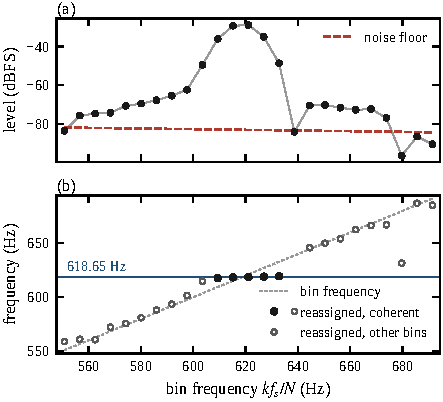
\includegraphics[width=\columnwidth]{fig_frame.pdf}
\caption{One frame of the recorded bowl of Section~\ref{sec:bowl} ($t = 20.21\s$) around the partial \texttt{D\#5-11}. (a)~Bin levels and noise floor. (b)~Reassigned frequency of each bin; filled: bins within $0.45$ bin of the peak's value. The single-frame value, $618.65\Hz$, differs from the window estimate, $618.46\Hz$, because the partial is a beating pair (Fig.~\ref{fig:zoom}b).}
\label{fig:frame}
\end{figure}

\section{Choice of the analysis window}
\label{sec:window}

A recording of a bowl contains strikes, rubbing, handling noise and silence. The partials are best measured on the free ring-out after a strike, before the next excitation, over a time long enough for split modes to be resolved.

\subsection{Attacks}

Two second-order Butterworth high-pass filters, at $150\Hz$ and $1\,\mathrm{kHz}$, feed block energies $E_b[j]$ over blocks of $5\ms$. Block $j$ starts an attack if, in either band, $E_b[j]$ exceeds the mean energy of blocks $j-24,\dots,j-4$ by $J_b$, with $J = 10\dB$ in the $150\Hz$ band and $12\dB$ in the $1\,\mathrm{kHz}$ band, provided the $150\Hz$ band lies above $-75\dB$ and no attack occurred in the preceding $0.3\s$. The low band follows the overall level; the high band isolates the broadband click of the mallet, which the low band misses when the bowl is still sounding from an earlier strike. The attack is placed at the start of the block preceding the one that detects it, and its strength is the largest energy of the $150\Hz$ band in the following $100\ms$. Energy-based detectors of this kind are reviewed in~\cite{Bello}.

\subsection{Candidates and score}

Each attack opens a candidate window starting with the first frame that begins at least $15\ms$ after it and lasting at most $T_{\max} = 5\s$. A later attack ends the window unless it is more than $3\dB$ weaker than the window's own attack, so that light touches during the ring-out do not cut it short. Sustained sounds without attacks are covered by windows of length $T_{\max}$ overlapping by half; such a window is discarded if it contains an attack, since it would mix two excitations. Each candidate is analysed as in Sections~\ref{sec:partials} and~\ref{sec:split} and scored by
\begin{equation}
S = \sum_{p \in \mathcal{L}} c_p\, q_p^2,\qquad q_p = \sst(\widetilde{\mathrm{SNR}}_p;\, 8\dB, 45\dB),
\label{eq:score}
\end{equation}
where $\mathcal{L}$ is the set of partials that would be listed (Section~\ref{sec:conf}), $c_p$ the confidence and $\widetilde{\mathrm{SNR}}_p$ the median SNR of partial $p$, and $\sst(x;a,b)$ the smoothstep function, $0$ below $a$, $1$ above $b$ and $3u^2-2u^3$ with $u = (x-a)/(b-a)$ in between. The quadratic weight lets a few partials measured at high SNR outscore many weak ones, so that a quiet passage rich in marginal partials does not displace a strike. Windows after an attack receive a factor 1.15. The best window is retained, its end is moved back to the last frame in which a listed partial is present (but not below $0.5\s$), and it is analysed again.

\section{Partials}
\label{sec:partials}

\subsection{Tracking}

Within the window, peaks are linked frame by frame, strongest first, to the nearest active track whose reference frequency lies within $\max(0.5\ \text{bin}, 25\ct)$; the reference follows the track with a smoothing factor of $0.3$. A track ends after a gap of $0.12\s$, and tracks of fewer than three frames are discarded~\cite{McAulay,SMS}. Tracks whose median frequencies are less than two bins apart, which cannot be distinct peaks of one frame, are merged, as are tracks within $12\ct$ that overlap in time by less than a quarter of their length; where several tracks share a frame, the strongest peak is kept. A partial within $4.5$ bins of one at least $25\dB$ stronger is removed as a side lobe or coding artefact, and partials shorter than $80\ms$ are dropped.

\subsection{Frequency, spread and uncertainty}

Let $f_i$, $i = 1,\dots,n$, be the frame frequencies of a partial and $\mathrm{SNR}_i$ its peak SNRs. With weights $w_i = 10^{\min(\mathrm{SNR}_i,\,45\,\mathrm{dB})/10}$, let $f_m$ be the weighted median and $d_i = 1200\log_2(f_i/f_m)$ the deviations in cents. The robust spread is the weighted median absolute deviation, scaled to the standard deviation of a normal distribution~\cite{Rousseeuw},
\begin{equation}
\sigma_R = 1.4826\, \max\Bigl(0.03\ct,\ \operatorname{wmed}_i |d_i|\Bigr).
\end{equation}
A median is essential for beating partials: at the minima of a beat, where the frequency of an unresolved pair swings furthest, the level and therefore the weight is lowest. The frequency of the partial is the weighted mean, in cents, of the $f_i$ with $|d_i| \le \max(3\sigma_R, 1.5\ct)$, and its standard uncertainty is
\begin{equation}
u = \frac{\sqrt{\sigma_R^2 + 0.05\ct^2}}{\sqrt{\max(1, D/T_N)}},
\label{eq:unc}
\end{equation}
where $D = nH/f_s$ is the duration and $T_N = N/f_s$, so that $D/T_N$ counts non-overlapping frames. The constant term is a floor that keeps $u$ from vanishing; it limits $u$ to about $0.04\ct$ for long, stable partials. For a beating partial the deviations recur at the beat period, so that $D/T_N$ overstates the number of independent values; $u$ then describes the scatter of the frame estimates, and the zoom spectrum of Section~\ref{sec:split} usually does better for a resolved pair (Section~\ref{sec:synth}). A partial without a resolved partner may be a pair measured as a blend of its two modes. For such a partial, the shift that the zoom spectrum makes to the frequency, or half the beat rate measured from the envelope, whichever is larger, is added to $u$ in quadrature, both in cents.

\subsection{Confidence}
\label{sec:conf}

The confidence of a partial is the product
\begin{equation}
\begin{split}
c = {}& \sst(\widetilde{\mathrm{SNR}};6\dB,24\dB)\,\bigl(1 - e^{-D/0.2\,\mathrm{s}}\bigr)\\
&\times \sqrt{P}\; \frac{1}{1 + (\sigma_R/6\ct)^2}\, \sqrt{\rho}\; \beta .
\end{split}
\label{eq:conf}
\end{equation}
$P$ is the presence of the partial in its core interval, the shortest run of frames holding $90\,\%$ of its weight: the fraction of those frames in which it was found. $\rho$ is the fraction of the weight carried by frames within $\max(6 \cdot 1.4826\, \mathrm{MAD}, 3\ct)$ of $f_m$, MAD being the unweighted median of $|d_i|$ (at least $0.3\ct$). $\beta$ is $1$, or $0.05$ for background (Section~\ref{sec:bg}). Each factor lies in $[0,1]$ and penalises one way of being spurious: a weak peak, a brief event, an intermittent track, a wandering frequency, a track assembled from unrelated peaks, a tone that does not belong to the instrument. A partial is listed if $c \ge \theta$ ($0.7$ by default), its peak level is within $60\dB$ of that of the strongest partial with $c \ge 0.3$, and its duration is at least $D_{\min}$ ($1\s$ by default). The duration factor alone reaches $0.63$ at $0.2\s$ and $0.99$ at $1\s$; $D_{\min}$ excludes events that are measured confidently but are too brief to matter musically.

\subsection{Background}
\label{sec:bg}

A steady tone from the room or from electronics can be strong, stable and long, and pass every test above. A partial is marked as background if it was already present before the strike: a peak lies within $\max(1.5\ \text{bins}, 20\ct)$ of its frequency in at least half of the frames of the $0.5\s$ before the attack, its level in the first $0.4\s$ after the attack exceeds the highest of those levels by less than $4\dB$, and the slope of its level over the window is below $0.3\dB/\mathrm{s}$ in magnitude. A second test, which also serves windows without an attack, takes the quietest $10\,\%$ of the frames of the signal as reference, provided they are at least $10\dB$ quieter than the window, and requires the median level of the partial to exceed its median level there by less than $6\dB$, with the same conditions on presence and slope.

\section{Split modes and beating}
\label{sec:split}

In an axisymmetric shell each mode with nodal meridians is a degenerate pair; departures from symmetry in shape, thickness or material split the pair into two modes a fraction of a hertz to a few hertz apart, and their sum beats~\cite{FletcherRossing,Inacio,Terwagne}. The main lobe of the analysis window spans $\pm 23\Hz$ at $48\,\mathrm{kHz}$, so each frame sees the pair as one peak whose frequency and level oscillate at the beat rate, and the frequency of Section~\ref{sec:partials} is a weighted average of the two modes.

\subsection{Zoom spectrum}

For each partial with $c \ge 0.2$ that is not background, the core interval, limited to the window and to $5\s$, defines a segment of length $T \ge 0.8\s$. The segment is weighted by a Blackman--Harris window of length $T$, shifted to zero frequency by multiplication with $e^{-2\pi i f n/f_s}$, $f$ being the tracked frequency, low-pass filtered and decimated by $M = \mathrm{round}(f_s/400\Hz)$ with a triangular kernel spanning $2M$ samples (moving averages of lengths $M$ and $M+1$ in cascade, with nulls near multiples of $f_s/M \approx 400\Hz$), and Fourier transformed directly on a grid of spacing $\min(0.05\Hz, 0.2/T)$ over $\pm B$,
\begin{equation}
B = \max\bigl(4/T,\ \min(12\Hz,\ 0.45\,\Delta)\bigr),
\end{equation}
$\Delta$ being the distance to the nearest other partial with $c \ge 0.2$ that is not background. This is the zoom transform by complex demodulation~\cite{Yip,Randall}; evaluated on the narrow grid it costs about $10^6$ operations per partial. The highest peak, refined by quadratic interpolation, replaces the tracked frequency if it lies within $\max(1\Hz, 8\ct, 0.8\ \text{bin})$ of it, the range over which an unresolved pair can pull the tracked value. A second peak at least $3/T$ from the first, no more than $\min\bigl(25\dB, \max(10\dB, \widetilde{\mathrm{SNR}} - 10\dB)\bigr)$ below it and not within two grid steps of $\pm B$ is reported as the partner mode; the beat rate is the distance between the two. A resolved pair accounts for the frame-to-frame wobble of the frequency, and the stability factor of~\eqref{eq:conf} is then raised to at least $0.95$.

\subsection{Envelope beat}

A pair that decays within about a second cannot be resolved, since the zoom window's main lobe spans $\pm 4/T$, but it still modulates the level. Over the whole track of the partial (at least $0.6\s$; the core interval of a fast-decaying partial is too short), its level is interpolated across gaps and detrended by a straight line in dB, i.e.\ by an exponential decay. If the residual $r_j$ spans at least $2\dB$ between its 5th and 95th percentiles, its normalised autocorrelation
\begin{equation}
\gamma(L) = \frac{n}{n-L}\, \frac{\sum_{j} r_j r_{j+L}}{\sum_j r_j^2}
\end{equation}
is searched for its highest local maximum between lags of $0.15\s$ and $\min(2.5\s, nH/2f_s)$. If that maximum reaches $0.5$ and the track spans at least two of its lags, the beat rate is the inverse of the lag, refined by parabolic interpolation, and the uncertainty of the partial is widened as described in Section~\ref{sec:partials}.


\section{Display and audibility}
\label{sec:display}

\subsection{Spiral}

As in the Snail~\cite{HelieSnail}, the spectrum is drawn on a spiral with one turn per octave, the pitch helix~\cite{Drobisch,Shepard82} seen along its axis. A frequency $f$ is placed at
\begin{equation}
u = \log_2(f/f_{\mathrm{lo}}),\quad \theta = 2\pi u,\quad \rho = r_0 + \Delta r\, u,
\end{equation}
with the angle $\theta$ measured clockwise from the top and $f_{\mathrm{lo}}$ the C at the bottom of the displayed range (C2, over seven octaves, by default). The C line points upwards, and the twelve pitch classes of the equal-tempered scale lie on twelve radial lines.

\subsection{Reassigned spectrum}

For the window, the power of each bin is moved to its reassigned frequency~\eqref{eq:reassd} and accumulated on a fixed grid of $2$-cent cells from C1 to C10: bin $k$ of frame $\ell$ adds $4|X_h[\ell,k]|^2/(N\sum_n h[n]^2)$ to the cell nearest $\hat f[\ell,k]$, provided $|\hat f[\ell,k] - k f_s/N| \le 3.5$ bins, i.e.\ the estimate lies inside the main lobe, and the bin lies within $112\dB$ of the frame maximum. The factor makes the cells of a stationary sinusoid of amplitude $A$ sum to $A^2$. This is the reassigned spectrogram of~\cite{Kodera78,AugerFlandrin}, reduced to its frequency coordinate. The cells are averaged over the frames of the window (or their maximum is taken, as an option), and the cell of each listed partial is raised to the partial's peak level, so that partials that die out early in the window keep their height. Cell levels are mapped to $v_c \in [0,1]$ over a display range below the maximum ($60\dB$), widened to lenses,
\begin{equation}
v'_c = \max_j\, \bigl( v_{c+j} - (2j/W)^2 \bigr),
\end{equation}
of half-width $W\sqrt{v}$ cents ($W = 22\ct$), and drawn as a band of half-thickness $0.47\,\Delta r\, v'_c$ across the spiral, coloured by $v'_c$ (Fig.~\ref{fig:spiral}).

\subsection{Audibility}

The level of a partial says little about how prominently it is heard. Each listed partial is weighted by the equal-loudness contour at $60$ phon of ISO~226:2003~\cite{ISO226},
\begin{equation}
w_p = L_p - \bigl(L_{60}(f_p) - 60\dB\bigr),
\end{equation}
$L_p$ being its peak level relative to the strongest partial and $L_{60}(f)$ the sound pressure level of the contour, computed from the standard's formula at its 29 frequencies and interpolated in $\log f$. Relative to the largest $w_p$, a partial is \emph{dominant} above $-10\dB$, \emph{clear} above $-25\dB$, \emph{faint} above $-40\dB$ and \emph{very faint} below. It is moved one class down if a partial at least $15\dB$ stronger in $w$ lies within one unit of the ERB-number scale~\cite{GlasbergMoore},
\begin{equation}
E(f) = 21.4\log_{10}(1 + 0.00437 f),
\end{equation}
as a crude allowance for masking. The calibration of a recording is unknown, so $60$ phon stands for a moderate listening level; the classes are a guide to prominence, not a loudness model.

\begin{table*}[t]
\centering
\caption{Recorded bowl, window $18.62$--$23.80\s$, default settings ($\theta = 0.7$, $D_{\min} = 1\s$, $f_{\mathrm{A4}} = 440\Hz$), as exported by the implementation. Level: peak level relative to the strongest partial; $u$: standard uncertainty~\eqref{eq:unc}, widened for \#4 as described in Section~\ref{sec:partials}.}
\label{tab:bowl}
\small
\begin{tabular}{@{}clrrrlcrrr@{}}
\toprule
\# & note & frequency (Hz) & ratio & level (dB) & audibility & confidence & $u$ (cents) & beat (Hz) & partner (Hz)\\
\midrule
1 & \texttt{A\#3+42} & 238.87 & 1.000 & $-3.3$ & clear & 0.99 & 0.14 & 1.11 & 237.76\\
2 & \texttt{D\#5-11} & 618.46 & 2.589 & $0.0$ & dominant & 0.99 & 0.10 & 0.95 & 619.42\\
3 & \texttt{D6-47} & 1143.27 & 4.786 & $-3.2$ & dominant & 1.00 & 0.06 & 0.84 & 1142.42\\
4 & \texttt{A6+38} & 1799.24 & 7.532 & $-14.4$ & clear & 0.99 & 1.45 & 3.01 & --\\
\bottomrule
\end{tabular}
\end{table*}

\section{Microphone input}
\label{sec:mic}

The microphone signal reaches the analysis through an audio worklet in blocks of 1024 samples and is kept in a ring buffer of $20\s$. Frames are analysed as they arrive and feed the live display. An attack opens a capture, which is closed by the next attack of comparable strength, after $T_{\max}$, or, once it is $1\s$ old, when no confident partial has been seen for $0.6\s$. While no capture is open and confident partials are sounding, a capture of length $T_{\max}$ is also taken every $2.5\s$, for sustained sounds; unlike the windows of Section~\ref{sec:window}, these are not required to be free of attacks. Each capture is analysed as in Sections~\ref{sec:window}--\ref{sec:split}, with the quietest frames of the last $30\s$ as background reference and the zoom spectra computed from the ring buffer, and its end is trimmed as in Section~\ref{sec:window} without a second analysis. Captures without a listed partial are discarded. The best capture by~\eqref{eq:score} is shown; once there are two or more, each partial is reported with the number of captures in which it, or the other mode of its pair, was found within $15\ct$.

\section{Evaluation}
\label{sec:eval}

\subsection{Single-frame accuracy}
\label{sec:accuracy}

A sinusoid of random phase, with frequency uniform over one bin above $1\,\mathrm{kHz}$, in white Gaussian noise, was analysed in one frame ($f_s = 48\,\mathrm{kHz}$, $N = 8192$, 300 trials per SNR, the SNR per sample being $A^2/2\sigma^2$ for amplitude $A$ and noise variance $\sigma^2$). Fig.~\ref{fig:accuracy} compares the root-mean-square error of the reassigned frequency~\eqref{eq:reassd} at the highest bin with that of quadratic interpolation of the log magnitude~\cite{PARSHL,AbeSmith}, and with the Cram\'er--Rao bound for a sinusoid observed over $N$ samples~\cite{RifeBoorstyn}. The reassigned frequency stays within a factor $2.1$ to $2.6$ of the bound from $-20$ to $45\dB$ SNR per sample (the processing gain of the frame, by which the ratio of the sinusoid's peak power to the noise power in a bin exceeds the SNR per sample, is $N/(2B_e) = 33\dB$, $B_e = 2.00$ bins being the equivalent noise bandwidth of the window~\cite{Harris}); the factor is the price of the window's taper. The interpolated estimate levels off at $0.023\ct$ (at most $0.032\ct$), the bias of the parabolic fit~\cite{AbeSmith}. Above $45\dB$ the reassigned estimate levels off at about $4\cdot10^{-4}\ct$ RMS ($2.5\cdot10^{-4}\Hz$), the limit set by the window's end values. With a decay time constant of $2\s$ the noise-free error remains below $7\cdot10^{-4}\ct$. Both estimators are far more precise than the tuning of a bowl requires; what limits the measurement in practice is the behaviour of the partials themselves, chiefly beating.

\begin{figure}[t]
\centering
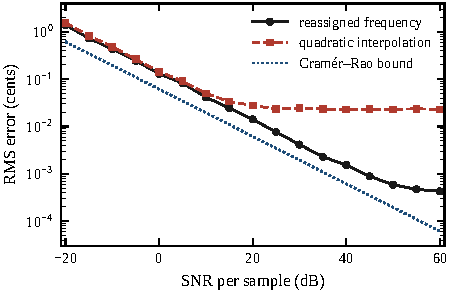
\includegraphics[width=\columnwidth]{fig_accuracy.pdf}
\caption{Single-frame frequency error for a sinusoid near $1\,\mathrm{kHz}$ in white noise ($N = 8192$, $f_s = 48\,\mathrm{kHz}$; 1 cent is $0.58\Hz$ here), against the Cram\'er--Rao bound~\cite{RifeBoorstyn}.}
\label{fig:accuracy}
\end{figure}

\subsection{Synthetic ring-outs}
\label{sec:synth}

Two struck bowls were synthesised as in~\eqref{eq:model}, each with a $3\ms$ noise burst for the strike at $t_0 = 3\s$. Table~\ref{tab:synth} gives the results with the default settings.

Case~A ($44.1\,\mathrm{kHz}$) has seven partials with time constants from $12.5$ to $1.7\s$, among them two split pairs, $280.20$/$283.90\Hz$ (amplitudes $0.05$/$0.03$) and $2314.00$/$2317.50\Hz$ ($0.02$/$0.01$), separated by about 17 and 16 times $1/T$; a steady background tone at $11926.8\Hz$ of amplitude $4\cdot10^{-4}$, present throughout; and white noise of standard deviation $3.5\cdot10^{-5}$, so that the median SNRs of the partials lie between 69 and $91\dB$. The attack is detected in the block containing $t_0$ and placed $8\ms$ before it, and the window $3.01$--$8.20\s$ is chosen. The frequencies of the five partials and of both partner modes are recovered to within $8\cdot10^{-6}\Hz$, the beat rates to $3\cdot10^{-6}\Hz$, and the partner levels as synthesised, $20\log_{10}0.6 = -4.4\dB$ and $20\log_{10}0.5 = -6.0\dB$. Before refinement the lower pair had been tracked at $280.84\Hz$, between its modes. The background tone is detected and its confidence reduced to $0.05$.

Case~B ($48\,\mathrm{kHz}$) takes parameters close to those of the recorded bowl of Section~\ref{sec:bowl}: four pairs with its frequencies and partner ratios, decaying at $1.1$, $0.8$, $4.8$ and $27\dB/\mathrm{s}$; the last has nearly equal modes $2.98\Hz$ apart ($1799.24$/$1802.22\Hz$, amplitude ratio $0.69$), in white Gaussian noise of standard deviation $0.003$ (median SNRs from 25 to $56\dB$). The three slower pairs are resolved, although their modes are only 3 to 5 times $1/T$ apart: the main modes are found within $0.0003$, $0.0000$ and $0.023\ct$ of the truth and the partners within $1.3$, $0.2$ and $40\,\mathrm{mHz}$, the last pair, at about $3/T$, being the hardest. Their uncertainties, $0.19$, $0.10$ and $0.06\ct$, computed from the frame-to-frame wobble, cover these errors. The fast pair is not resolved. It is reported at $1800.24\Hz$, between its modes and $0.97\ct$ above the stronger, with its beat of $2.98\Hz$ from the envelope and an uncertainty of $1.44\ct$. At half the noise the errors of the three resolved main modes fall below $0.001\ct$, and without noise all four pairs are resolved, to $3\cdot10^{-4}\ct$.

\begin{table}[t]
\centering
\caption{Synthetic ring-outs: synthesised and measured frequencies (Hz), confidence $c$ and uncertainty $u$ (cents). Partner modes are given below the main mode of each pair.}
\label{tab:synth}
\small
\setlength{\tabcolsep}{4.5pt}
\begin{tabular}{@{}rrrrl@{}}
\toprule
synthesised & measured & $c$ & $u$ & \\
\midrule
\multicolumn{5}{@{}l}{\emph{Case A}}\\
280.20 & 280.200\,00 & 0.94 & 0.84 & beat 3.700\\
283.90 & 283.900\,00 & & & partner, $-4.4\dB$\\
802.93 & 802.930\,00 & 1.00 & 0.04 & \\
1497.21 & 1497.210\,00 & 1.00 & 0.04 & \\
2314.00 & 2314.000\,00 & 0.99 & 0.11 & beat 3.500\\
2317.50 & 2317.500\,00 & & & partner, $-6.0\dB$\\
3277.39 & 3277.389\,99 & 1.00 & 0.04 & \\
11926.80 & 11926.800\,40 & 0.05 & 0.04 & background\\
\midrule
\multicolumn{5}{@{}l}{\emph{Case B}}\\
238.87 & 238.870\,0 & 0.97 & 0.19 & beat 1.109\\
237.76 & 237.761\,3 & & & partner, $-17.9\dB$\\
618.46 & 618.460\,0 & 0.99 & 0.10 & beat 0.960\\
619.42 & 619.419\,8 & & & partner, $-14.5\dB$\\
1143.27 & 1143.285\,2 & 1.00 & 0.06 & beat 0.905\\
1142.42 & 1142.380\,1 & & & partner, $-5.4\dB$\\
1799.24 & 1800.243\,4 & 0.99 & 1.44 & beat 2.978 (envelope)\\
1802.22 & & & & partner, unresolved\\
\bottomrule
\end{tabular}
\end{table}

\begin{figure}[t]
\centering
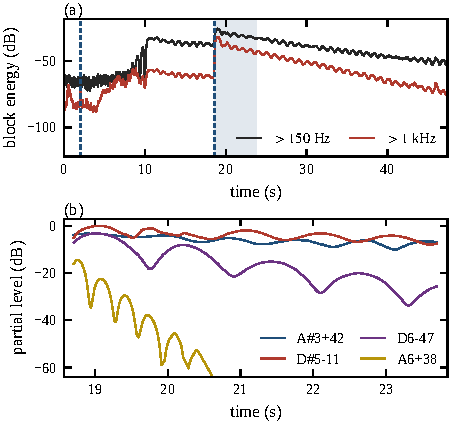
\includegraphics[width=\columnwidth]{fig_timeline.pdf}
\caption{Recorded bowl. (a)~Block energies of the onset detector over the whole recording; dashed: detected attacks; shaded: the selected window. (b)~Peak levels of the four listed partials in the window, relative to the strongest; the periodic dips are beats.}
\label{fig:timeline}
\end{figure}

\subsection{A recorded bowl}
\label{sec:bowl}

Figs.~\ref{fig:spiral}, \ref{fig:timeline} and~\ref{fig:zoom} and Table~\ref{tab:bowl} show the analysis of a $47\s$ recording of a singing bowl at $48\,\mathrm{kHz}$, its two channels averaged. Two attacks are detected (Fig.~\ref{fig:timeline}a): a light one at $2.0\s$ and a strike at $18.6\s$, $32\dB$ stronger; between $5$ and $11\s$ the level rises without an attack. The ring-out window $18.62$--$23.80\s$ scores $4.37$; the best sliding window, $20.05$--$25.23\s$ later in the same ring-out, scores $2.95$, and the best over the passage without a strike, $7.52$--$12.69\s$, $2.80$. Of the 109 partials formed in the window, four are listed, at frequency ratios $1 : 2.589 : 4.786 : 7.532$. Among the others, a partial at $2577.68\Hz$ has confidence $0.82$ but lasts $0.35\s$ and is excluded by $D_{\min}$; none of the rest exceeds $0.39$.

The three lower partials are split pairs (Fig.~\ref{fig:zoom}). Their partners lie $1.11$, $0.95$ and $0.84\Hz$ away and $17.9$, $14.5$ and $5.2\dB$ below the main mode. For an amplitude ratio $r$ the level of a pair swings by $20\log_{10}\bigl((1+r)/(1-r)\bigr)$, here $2.2$, $3.3$ and $10.7\dB$, close to the swings of the detrended level curves of Fig.~\ref{fig:timeline}b, $2.9$, $4.0$ and $10.3\dB$ between their 5th and 95th percentiles. The partial at $1799.24\Hz$ decays at $23\dB/\mathrm{s}$, against $0.8$ to $4.8\dB/\mathrm{s}$ for the others. Its zoom segment of $1.0\s$ cannot separate modes $3\Hz$ apart, and its beat of $3.01\Hz$ is measured from the envelope; its level swings by $14\dB$, which implies nearly equal modes (amplitude ratio about $0.67$), the situation of the fast pair of Case~B. Its uncertainty, $1.45\ct$, therefore includes half the beat rate. When the recording is played into the microphone path of Section~\ref{sec:mic}, the capture of this ring-out gives a zoom segment of $1.14\s$ for this partial, and the pair is resolved there, at $1799.22$ and $1802.17\Hz$, $0.8\dB$ apart. Refinement moved the tracked frequencies by $+0.02$, $+0.01$, $+0.11$ and $-1.11\Hz$.

\begin{figure}[t]
\centering
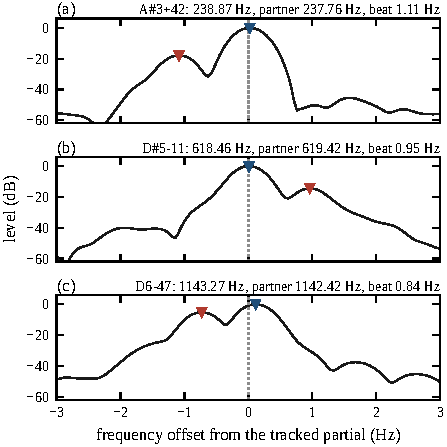
\includegraphics[width=\columnwidth]{fig_zoom.pdf}
\caption{Zoom spectra of the three lower partials of the recorded bowl over their core intervals ($T = 4.5$ to $4.7\s$). Blue: main mode, red: partner; dashed: the frequency tracked from the frames.}
\label{fig:zoom}
\end{figure}


\subsection{Computation}

A frame, two FFTs of $8192$ points and the peak analysis, takes $0.7$ to $0.8\ms$ in JavaScript (V8, Node.js~22) on one core of a cloud virtual machine, under $8\,\%$ of the hop of $10.7\ms$; the $47\s$ recording, $4430$ frames, is analysed with all candidate windows in about $5\s$.

\section{Relation to the Snail-Analyser}
\label{sec:snail}

Both methods estimate, for each analysis frequency, the frequency of the component in its spectral lobe, and use the estimate to sharpen a spiral display. They differ in how the estimate is formed, in what sharpens the display, and in what they deliver.

The Snail interpolates the STFT onto a logarithmic grid of analysis frequencies, typically 20 per semitone, with frames of $50\ms$ every $5\ms$~\cite{HelieTimbre}. Its frequency deviation is the change of the demodulated phase $\varphi_d(t,f) = \varphi(t,f) - 2\pi f t$ between successive frames, divided by $2\pi$ times the hop, and its display weights the loudness at each analysis frequency by the modulus of the low-pass filtered phasor $e^{i\varphi_d}$; this weighting contracts the lobe of a stationary component to a width set by the cut-off frequency and suppresses components that vary faster~\cite{HelieTimbre,HeliePatent}. The present method forms neither the demodulated phase nor a phase difference between frames. Its frequency estimate is the reassigned frequency~\eqref{eq:reassd} of a single frame, on the linear grid of the FFT, and its display is sharpened by moving power to that frequency, without a weighting by temporal consistency. As the hop tends to zero the two frequency estimates tend to the same quantity, the instantaneous frequency of the band-pass signal of the bin~\cite{Kodera78,AugerFlandrin}: the Snail evaluates it by a finite difference across frames, the present method analytically within one frame.

The two designs trade reactivity against measurement. The Snail follows vibrato and glissandi within tens of milliseconds, presents a clean image in noise through its constancy weighting, and adds tuning and harmonic-synchronicity indicators for performers~\cite{HelieTimbre}. The present method uses frames more than three times longer and reports partials only once a ring-out of at least $D_{\min}$ has been analysed; noise appears in its display at its reassigned frequencies, at low level, and is kept out of the list by the tests of Sections~\ref{sec:frame} and~\ref{sec:partials} rather than by a weighting of the image. In return it chooses its analysis window, gives each partial a confidence and a standard uncertainty, and resolves split modes a fraction of a hertz apart, which requires an observation of several seconds (Section~\ref{sec:split}); none of these is part of the published descriptions of the Snail~\cite{HelieSnail,HelieTimbre}.

\section{Conclusion}

The method measures the sustained partials of a struck bowl on the ring-out it selects itself, and states how far each measurement can be trusted. Its frequency estimates come from reassignment within single frames, which in continuous time is exact for an exponentially damped complex exponential, and which in noise stays within a factor of $2.1$ to $2.6$ of the Cram\'er--Rao bound; at that precision the measurement is governed by the instrument. Split modes that last long enough are resolved by a zoom spectrum over the ring-out, to within $0.03\ct$ with the parameters of the recorded bowl; a pair that decays too fast is reported as a blend of its modes, with its beat rate and a correspondingly wider uncertainty. The confidence~\eqref{eq:conf} and the minimum duration remove brief and unstable events, and background tones are recognised by their presence before the strike. The spiral display shows the reassigned spectrum from which the partials were measured, so that what the list reports can be seen. The implementation, a single HTML file, is released under the GNU General Public License, version 3 or later.

\small
\begin{thebibliography}{99}
\setlength{\itemsep}{1pt}

\bibitem{FletcherRossing}
N.~H. Fletcher and T.~D. Rossing, \emph{The Physics of Musical Instruments}, 2nd~ed. New York: Springer, 1998, ch.~21, ``Bells,'' pp.~675--707.

\bibitem{Inacio}
O.~Inácio, L.~L. Henrique, and J.~Antunes, ``The dynamics of Tibetan singing bowls,'' \emph{Acta Acust. united Ac.}, vol.~92, no.~4, pp.~637--653, 2006.

\bibitem{Terwagne}
D.~Terwagne and J.~W.~M. Bush, ``Tibetan singing bowls,'' \emph{Nonlinearity}, vol.~24, no.~8, pp.~R51--R66, 2011, doi:10.1088/0951-7715/24/8/R01.

\bibitem{HelieSnail}
T.~Hélie and C.~Picasso, ``The Snail: a real-time software application to visualize sounds,'' in \emph{Proc. 20th Int. Conf. Digital Audio Effects (DAFx-17)}, Edinburgh, UK, 2017, pp.~443--450.

\bibitem{HelieTimbre}
T.~Hélie, C.~Picasso, R.~Piéchaud, M.~Jousserand, and T.~Colinot, ``Real-time visualisation of the musical timbre based on the spectral estimates of the Snail-Analyser,'' in \emph{Proc. 26th Int. Conf. Digital Audio Effects (DAFx23)}, Copenhagen, Denmark, 2023, HAL: hal-04162814.

\bibitem{HeliePatent}
T.~Hélie (Centre National de la Recherche Scientifique), ``Analyse fréquentielle par démodulation de phase d'un signal acoustique'' (Frequency analysis by phase demodulation of an acoustic signal), Int. Patent Appl. WO~2015/189419~A1, 2015; European Patent EP~3\,155\,609~B1, 2019.

\bibitem{McAulay}
R.~J. McAulay and T.~F. Quatieri, ``Speech analysis/synthesis based on a sinusoidal representation,'' \emph{IEEE Trans. Acoust., Speech, Signal Process.}, vol.~ASSP-34, no.~4, pp.~744--754, 1986.

\bibitem{PARSHL}
J.~O. Smith and X.~Serra, ``PARSHL: an analysis/synthesis program for non-harmonic sounds based on a sinusoidal representation,'' in \emph{Proc. Int. Computer Music Conf.}, Champaign-Urbana, IL, USA, 1987, pp.~290--297.

\bibitem{SMS}
X.~Serra and J.~O. Smith, ``Spectral modeling synthesis: a sound analysis/synthesis system based on a deterministic plus stochastic decomposition,'' \emph{Computer Music J.}, vol.~14, no.~4, pp.~12--24, 1990.

\bibitem{Kodera76}
K.~Kodera, C.~de~Villedary, and R.~Gendrin, ``A new method for the numerical analysis of non-stationary signals,'' \emph{Phys. Earth Planet. Inter.}, vol.~12, no.~2--3, pp.~142--150, 1976.

\bibitem{Kodera78}
K.~Kodera, R.~Gendrin, and C.~de~Villedary, ``Analysis of time-varying signals with small BT values,'' \emph{IEEE Trans. Acoust., Speech, Signal Process.}, vol.~ASSP-26, no.~1, pp.~64--76, 1978.

\bibitem{AugerFlandrin}
F.~Auger and P.~Flandrin, ``Improving the readability of time-frequency and time-scale representations by the reassignment method,'' \emph{IEEE Trans. Signal Process.}, vol.~43, no.~5, pp.~1068--1089, 1995.

\bibitem{ISO16}
ISO~16:1975, \emph{Acoustics --- Standard tuning frequency (Standard musical pitch)}. Geneva: International Organization for Standardization, 1975.

\bibitem{Harris}
F.~J. Harris, ``On the use of windows for harmonic analysis with the discrete Fourier transform,'' \emph{Proc. IEEE}, vol.~66, no.~1, pp.~51--83, 1978.

\bibitem{FulopFitz}
S.~A. Fulop and K.~Fitz, ``Algorithms for computing the time-corrected instantaneous frequency (reassigned) spectrogram, with applications,'' \emph{J. Acoust. Soc. Am.}, vol.~119, no.~1, pp.~360--371, 2006.

\bibitem{FlanaganGolden}
J.~L. Flanagan and R.~M. Golden, ``Phase vocoder,'' \emph{Bell Syst. Tech. J.}, vol.~45, no.~9, pp.~1493--1509, 1966.

\bibitem{DesainteCatherine}
M.~Desainte-Catherine and S.~Marchand, ``High-precision Fourier analysis of sounds using signal derivatives,'' \emph{J. Audio Eng. Soc.}, vol.~48, no.~7/8, pp.~654--667, 2000.

\bibitem{AbeSmith}
M.~Abe and J.~O. Smith III, ``Design criteria for simple sinusoidal parameter estimation based on quadratic interpolation of FFT magnitude peaks,'' presented at the 117th AES Convention, San Francisco, CA, USA, 2004, Convention Paper 6256.

\bibitem{Bello}
J.~P. Bello, L.~Daudet, S.~Abdallah, C.~Duxbury, M.~Davies, and M.~B. Sandler, ``A tutorial on onset detection in music signals,'' \emph{IEEE Trans. Speech Audio Process.}, vol.~13, no.~5, pp.~1035--1047, 2005.

\bibitem{Rousseeuw}
P.~J. Rousseeuw and C.~Croux, ``Alternatives to the median absolute deviation,'' \emph{J. Amer. Statist. Assoc.}, vol.~88, no.~424, pp.~1273--1283, 1993.

\bibitem{Yip}
P.~C.~Y. Yip, ``Some aspects of the zoom transform,'' \emph{IEEE Trans. Comput.}, vol.~C-25, no.~3, pp.~287--296, 1976.

\bibitem{Randall}
R.~B. Randall, \emph{Frequency Analysis}, 3rd~ed. Nærum, Denmark: Brüel \& Kjær, 1987.

\bibitem{Drobisch}
M.~W. Drobisch, ``Über musikalische Tonbestimmung und Temperatur,'' \emph{Abh. math.-phys. Cl. Königl. Sächs. Ges. Wiss.}, vol.~2, pp.~1--120, 1855.

\bibitem{Shepard82}
R.~N. Shepard, ``Geometrical approximations to the structure of musical pitch,'' \emph{Psychol. Rev.}, vol.~89, no.~4, pp.~305--333, 1982.

\bibitem{ISO226}
ISO~226:2003, \emph{Acoustics --- Normal equal-loudness-level contours}. Geneva: International Organization for Standardization, 2003 (since revised as ISO~226:2023).

\bibitem{GlasbergMoore}
B.~R. Glasberg and B.~C.~J. Moore, ``Derivation of auditory filter shapes from notched-noise data,'' \emph{Hear. Res.}, vol.~47, no.~1--2, pp.~103--138, 1990.

\bibitem{RifeBoorstyn}
D.~C. Rife and R.~R. Boorstyn, ``Single-tone parameter estimation from discrete-time observations,'' \emph{IEEE Trans. Inf. Theory}, vol.~IT-20, no.~5, pp.~591--598, 1974.

\end{thebibliography}

\end{document}
